\documentclass{article}
\usepackage{amsmath}
\usepackage{enumerate}
\usepackage{fancyhdr} % Required for custom headers
\usepackage{lastpage} % Required to determine the last page for the footer
\usepackage{extramarks} % Required for headers and footers
\usepackage[usenames,dvipsnames]{color} % Required for custom colors
\usepackage{graphicx} % Required to insert images
\usepackage[tight,footnotesize]{subfigure} % Required for subfig
\usepackage{caption} % Required for subfig
\usepackage{hyperref} % Required for url
\usepackage{listings} % Required for insertion of code
\usepackage{courier} % Required for the courier font
\usepackage{lipsum} % Used for inserting dummy 'Lorem ipsum' text into the template
\topmargin=-0.45in
\evensidemargin=0in
\oddsidemargin=0in
\textwidth=6.5in
\textheight=9.0in
\headsep=0.25in
\linespread{1.1} % Line spacing
\pagestyle{fancy}
\lhead{\hmwkAuthorName} % Top left header
% \chead{\hmwkClass\ (\hmwkClassInstructor\ \hmwkClassTime): \hmwkTitle} % Top center head
\chead{\hmwkClass\ : \hmwkTitle} % Top center head
\rhead{\firstxmark} % Top right header
\lfoot{\lastxmark} % Bottom left footer
\cfoot{} % Bottom center footer
\rfoot{Page\ \thepage\ of\ \protect\pageref{LastPage}} % Bottom right footer
\renewcommand\headrulewidth{0.4pt} % Size of the header rule
\renewcommand\footrulewidth{0.4pt} % Size of the footer rule
\setlength\parindent{0pt} % Removes all indentation from paragraphs

% Define floor and ceiling
\def\lc{\left\lceil}   
\def\rc{\right\rceil}
\def\lf{\left\lfloor}   
\def\rf{\right\rfloor}

% Set your language 
%\lstset{language=Java}
\definecolor{codegreen}{rgb}{0,0.6,0}
\definecolor{codegray}{rgb}{0.5,0.5,0.5}
\definecolor{codepurple}{rgb}{0.58,0,0.82}
\definecolor{backcolour}{rgb}{0.95,0.95,0.92}
 
\lstdefinestyle{mystyle}{
    backgroundcolor=\color{backcolour},   
    commentstyle=\color{codegreen},
    keywordstyle=\color{magenta},
    numberstyle=\tiny\color{codegray},
    stringstyle=\color{codepurple},
    basicstyle=\footnotesize,
    breakatwhitespace=false,         
    breaklines=true,                 
    captionpos=b,                    
    keepspaces=true,                 
    numbers=left,                    
    numbersep=8pt,                  
    showspaces=false,                
    showstringspaces=false,
    showtabs=false,                  
    tabsize=2
}
\lstset{style=mystyle}

% Header and footer for when a page split occurs within a problem environment
\newcommand{\enterProblemHeader}[1]{
\nobreak\extramarks{#1}{#1 continued on next page\ldots}\nobreak
\nobreak\extramarks{#1 (continued)}{#1 continued on next page\ldots}\nobreak
}

% Header and footer for when a page split occurs between problem environments
\newcommand{\exitProblemHeader}[1]{
\nobreak\extramarks{#1 (continued)}{#1 continued on next page\ldots}\nobreak
\nobreak\extramarks{#1}{}\nobreak
}

\setcounter{secnumdepth}{0} % Removes default section numbers
\newcounter{homeworkProblemCounter} % Creates a counter to keep track of the number of problems

\newcommand{\homeworkProblemName}{}
\newenvironment{homeworkProblem}[1][Problem \arabic{homeworkProblemCounter}]{ % Makes a new environment called homeworkProblem which takes 1 argument (custom name) but the default is "Problem #"
\stepcounter{homeworkProblemCounter} % Increase counter for number of problems
\renewcommand{\homeworkProblemName}{#1} % Assign \homeworkProblemName the name of the problem
\section{\homeworkProblemName} % Make a section in the document with the custom problem count
\enterProblemHeader{\homeworkProblemName} % Header and footer within the environment
}{
\exitProblemHeader{\homeworkProblemName} % Header and footer after the environment
}

\newcommand{\problemAnswer}[1]{ % Defines the problem answer command with the content as the only argument
\noindent\framebox[\columnwidth][c]{\begin{minipage}{0.98\columnwidth}#1\end{minipage}} % Makes the box around the problem answer and puts the content inside
}

\newcommand{\homeworkSectionName}{}
\newenvironment{homeworkSection}[1]{ % New environment for sections within homework problems, takes 1 argument - the name of the section
\renewcommand{\homeworkSectionName}{#1} % Assign \homeworkSectionName to the name of the section from the environment argument
\subsection{\homeworkSectionName} % Make a subsection with the custom name of the subsection
\enterProblemHeader{\homeworkProblemName\ [\homeworkSectionName]} % Header and footer within the environment
}{
\enterProblemHeader{\homeworkProblemName} % Header and footer after the environment
}

\newlength{\tabcont}

\newcommand{\tab}[1]{%
\settowidth{\tabcont}{#1}%
\ifthenelse{\lengthtest{\tabcont < .25\linewidth}}%
{\makebox[.25\linewidth][l]{#1}\ignorespaces}%
{\makebox[.5\linewidth][l]{\color{red} #1}\ignorespaces}%
}%
%----------------------------------------------------------------------------------------
%	NAME AND CLASS SECTION
%----------------------------------------------------------------------------------------

\newcommand{\hmwkTitle}{Homework\ \#1} % Assignment title
\newcommand{\hmwkDueDate}{Monday,\ January\ 1,\ 2012} % Due date
\newcommand{\hmwkClass}{Fundamental Algorithms} % Course/class
\newcommand{\hmwkClassTime}{} % Class/lecture time
\newcommand{\hmwkClassInstructor}{Prof. Joel Spencer} % Teacher/lecturer
\newcommand{\hmwkAuthorName}{Songxiao Zhang, N10224459} % Your name

%----------------------------------------------------------------------------------------
%	TITLE PAGE
%----------------------------------------------------------------------------------------

\title{
\textmd{\textbf{\hmwkClass:\ \hmwkTitle}}\\
}
\author{\textbf{\hmwkAuthorName}}

\begin{document}

\maketitle

%----------------------------------------------------------------------------------------
%	TABLE OF CONTENTS
%----------------------------------------------------------------------------------------

%\setcounter{tocdepth}{1} % Uncomment this line if you don't want subsections listed in the ToC

%\newpage
%\tableofcontents
%\newpage

%----------------------------------------------------------------------------------------
%	PROBLEM 1
%----------------------------------------------------------------------------------------
\begin{homeworkProblem}
The running time of HEAP-INCREASE-KEY(A, i , key) is not related to the total number of nodes but the number of nodes from the they to the root. The number of levels between the root and the key is 8 because
$$ 256 = 2^8 < 300, 300 < 2^9 = 512 $$

\begin{enumerate}[a.]
    \item So the maximum number of exchanges is 8 when $key > A[1]$. 
    \item The minimum number of changes is 0 when $A[key] \leq A[[key]]$
\end{enumerate}
\end{homeworkProblem}

%----------------------------------------------------------------------------------------
%	PROBLEM 2
%----------------------------------------------------------------------------------------
\begin{homeworkProblem}
The number of exchanges is related to the height of the tree. $50 \ million = 5 * 10^7$, 
$$2^{25} < 5 * 10^7 < 2^{26}, 2^{8} < 300 < 2^9$$
The heap height is 25. H[300] is is in level 8. 

\begin{enumerate}[a.]
    \item The maximum number of exchanges is 17 when there is at least a leaf node under subheap of H[300] has a value larger than H[300]. That is $25-8 = 17$
    \item The minimum number of changes is 0 when $A[1].left \leq 300$ and $A[1].right \leq 300$
\end{enumerate}
\end{homeworkProblem}


%----------------------------------------------------------------------------------------
%	PROBLEM 3
%----------------------------------------------------------------------------------------
\begin{homeworkProblem}
Since $1023 = 2^{10} - 1$, H is a fully-loaded heap with the height of 9. There are $\frac{1023+1}{2} = 512$ leaf nodes and $\frac{512}{2} = 256$  nodes of leaf nodes. The leaf nodes are indexed from $511$ to $1023$ where $1023-512=511$ and the height of the heap is 8. 
          
\begin{enumerate}[a.]
    \item $x$ can be H[2], H[3], H[4], H[5], H[6]. $x$ cannot be the root since the root is the smallest. 
          $x$ can be one of the child of root H[2] and H[3]. If H[2] or H[3] is bigger than $x$, $x$ can be 
          the child of the smaller one between H[2] and H[3].
    \item Yes, $H[700]$ can be the largest element. As mentioned above, the leaf nodes are indexed 
          from $511$ to $1023$ therefore $H[700]$ can be a leaf node and so it can be the 
          largest element. 
    \item No, $y$ cannot be the smallest one because $H[700]$ is not the root. The root is $H[1]$. 
    \item \texttt{Bonus question}: The height of $H[700]$ is on the $8^{th}$-level. 
          Based on the MAX-HEAP property, all s must smaller than their children and so only the elements above 
          $H[700]$ must be smaller than $H[700]$. The index of $H[700]$ can range from 9 to 700. In other words, $i$ can 
          have $700-8=692$ possible values. 
\end{enumerate}

% \begin{enumerate}[a.]
%     \item $x$ can be any leaf node; or a  of two leaf nodes cause $x$ still has two children 
%           nodes that have smaller values. The number of last level node positions is 
%           $$\lfloor \frac{1023+1}{2} \rfloor = 512$$ The number of second last level node positions is 
%           $$\lfloor \frac{1023+1}{} \rfloor = 256$$
%           There are $256 + 512 = 768$ possible positions for $x$. 
%     \item No, $y$ cannot be the largest one because $H[700]$ is not the root. The root is $H[1]$. 
%     \item Yes, $H[700]$ can be the smallest element. As mentioned above, the leaf nodes are indexed 
%           from $511$ to $1023$ therefore $H[700]$ can be a leaf node and so it can be the 
%           smallest element. 
%     \item \texttt{Bonus question}: The height of $H[700]$ is on the $8^{th}$-level. 
%           Based on the MAX-HEAP property, all s must larger than their children and so only the elements above 
%           $H[700]$ must be larger than $H[700]$. The rank of $H[700]$ can range from 9 to 700. In other words, $i$ can 
%           range from $1st$ to $700-8=692$-th smallest element. 
% \end{enumerate}
\end{homeworkProblem}

%----------------------------------------------------------------------------------------
%	PROBLEM 4
%----------------------------------------------------------------------------------------
\begin{homeworkProblem}
    \begin{figure}[h!]
        \centering
        \subfigure[]{\label{}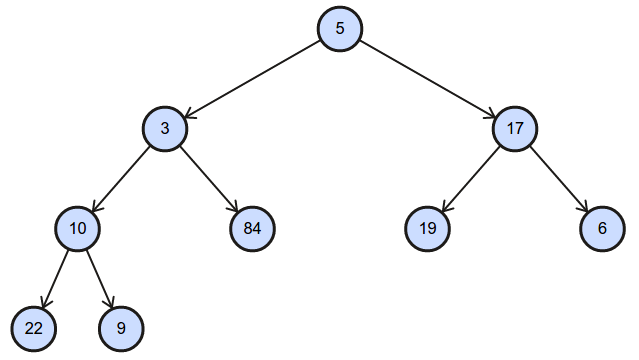
\includegraphics[width=0.45\textwidth]{hw1/1.png}}
        \subfigure[]{\label{}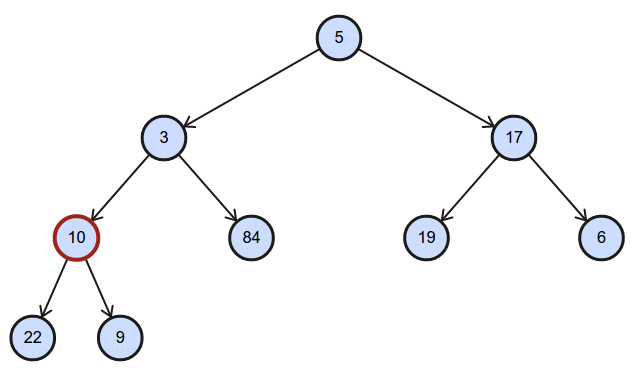
\includegraphics[width=0.45\textwidth]{hw1/2.png}}
        \subfigure[]{\label{}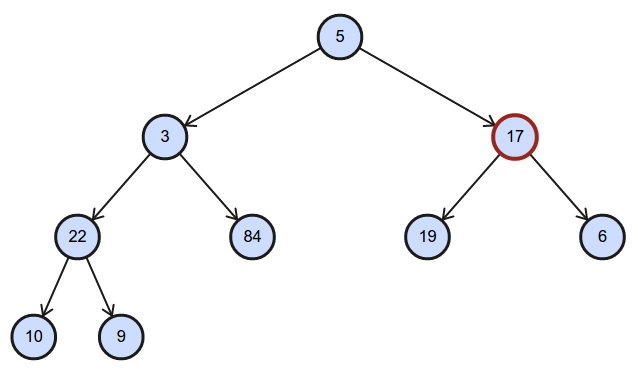
\includegraphics[width=0.45\textwidth]{hw1/3.png}}
        \subfigure[]{\label{}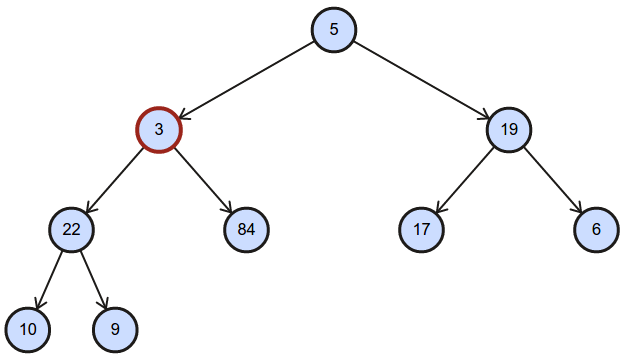
\includegraphics[width=0.45\textwidth]{hw1/4.png}}
        \subfigure[]{\label{}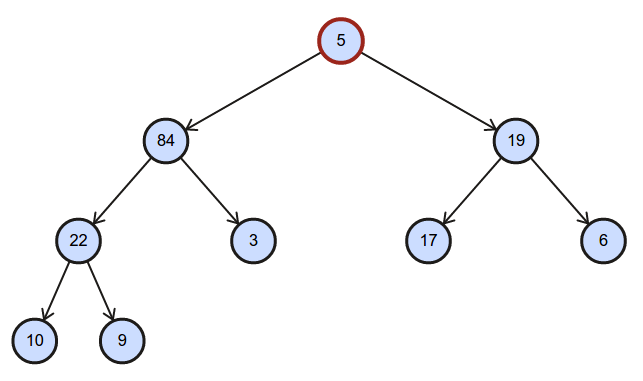
\includegraphics[width=0.45\textwidth]{hw1/5.png}}
        \subfigure[]{\label{}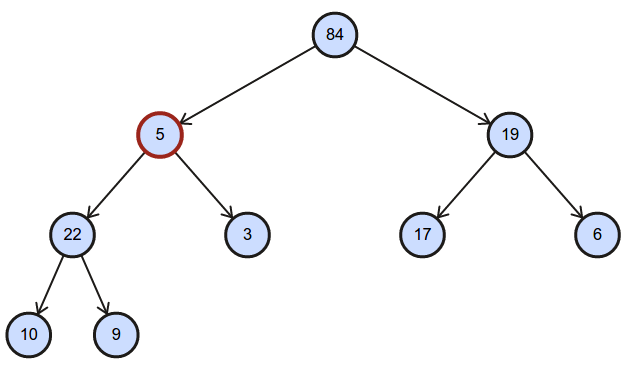
\includegraphics[width=0.45\textwidth]{hw1/6.png}}
        \subfigure[]{\label{}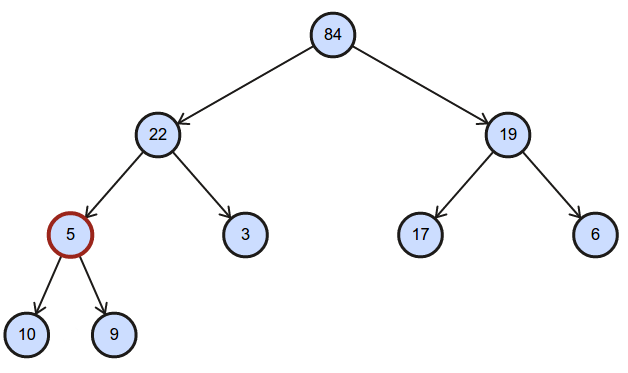
\includegraphics[width=0.45\textwidth]{hw1/7.png}}
        \subfigure[]{\label{}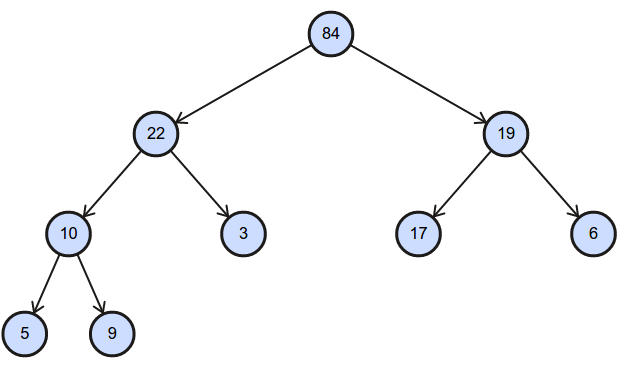
\includegraphics[width=0.45\textwidth]{hw1/8.png}}
        \caption{\textbf{a.} Fill the binary tree with array elements; 
                 \textbf{b.} Pick the first element in the 2nd last row, 
                    $\lfloor \frac{A.size+1}{2} \rfloor\}$. Swap the element
                    and its child if its value is smaller ($10<22$)
                 \textbf{c-g.} Move to the previous element by index, repeat b.
                 \textbf{h.} When complete b. at the root (A[1]), the process halt}
        \label{fig:flow}
    \end{figure} 

There are two orders to consider \textbf{Figure \ref{fig:flow}}. 
The graphs are generated by Visio. 
%\url{http://btv.melezinek.cz/}
\begin{enumerate}
    \item BUILD-MAX-HEAP(A) traverses from $\lfloor {A.length/2} \rfloor$ to $1$
    \item In each run of BUILD-MAX-HEAP(A), MAX-HEAPIFY(A, i) traverses from  to child. (Note: 
          MAX-HEAPIFY(A, i) compare twice but only swap once)
\end{enumerate}

\end{homeworkProblem}

%----------------------------------------------------------------------------------------
%	PROBLEM 5
%----------------------------------------------------------------------------------------
\begin{homeworkProblem}
% Delete a node from heap is requires its children to be the children as its  and maintain MAX-HEAP. 

HEAP-DELETE(A,t)
\begin{lstlisting}[frame=single]
if(t > A.heap_size)
    error "node doesn't exist in heap"
if(A[[t]] < A[A.heap_size])
    HEAP-INCREASE-KEY(A, t, A[A.heap_size])     //make sure upper levels still heap
else A[t] = A[A.heap_size]                      //swap last and t-th element
A.heap_size = A.heap_size - 1                   //remove last element
MAX-HEAPIFY(A, t)                               //make sure lower levels still heap
\end{lstlisting}

I tried to keep exchanging the missing element and its child and maintain MAX-HEAP. But it could result in removing an element in the middle of the last row then the heap is not a complete binary tree. Therefore, putting the last element in the missing place is needed. \\

But there 2 points that could cause trouble: when A[t] is deleted, in \textbf{Line 5}, the new sub-heap rooted at A[t] needs to be heapify if A[A.heap\_size] \textless A[t].child; if A[A.heap\_size] \textgreater A[t], the upper heap also needs to swap elements, which can be solved by HEAP-INCREASE-KEY(A, t, A[A.heap\_size]) or MAX-HEAP-INSERT(A, A[A.heap\_size]). We couldn't use HEAP-INCREASE-KEY(A, t, A[A.heap\_size]) directly like the MAX-HEAPIFY(A, t) because HEAP-INCREASE-KEY(A, t, A[A.heap\_size]) would halt when t is greater than A[A.heap\_size]. 
\end{homeworkProblem}

%----------------------------------------------------------------------------------------
%	PROBLEM 6
%----------------------------------------------------------------------------------------
\begin{homeworkProblem}

\begin{enumerate}[a.]
    \item No exchange when the array is in an increasing order. Max heap is a semi-ordered array, and an increasing 
          order array is a built heap. 
    \item There are 120 exchanges. From bottom-up as BUILD-MAX-HEAPIFY does $\lfloor {A.length/2} \rfloor$ to $1$, the 2nd last level has
          $(A.length + 1)/$ nodes MAX-HEAPIFY(A, i) 1 time, the 3rd last level has $(A.length + 1)/2^3$ nodes 
          MAX-HEAPIFY(A, i) 2 times and so on until the root. Each MAX-HEAPIFY(A, i) involves 1 swapping. 
          $$ 2^5 \times 1 + 2^4 \times 2 + 2^3 \times 3 + \ldots + 1 \times 6 = 120 $$
          Note: MAX-HEAPIFY(A, i) compare twice but only swap once
\end{enumerate}

\end{homeworkProblem}

\vfill

\textbf{Reference claim}: When I had no clue on the bonus question, Mr. Wu Jon gave a pointer on that $i$ was not the index of heap (I was totally trapped in there). 
\end{document}